\clearpage
\section{Background}
\label{sec:background}

This section describes the used techniques in this study. First we describe multimodal machine learning, and their key challenges. Followed by background information on object detection, and the evolution of models until the current state-of-art YOLOv5. Finally, we explain some key signal processing operations that are often applied on accelerometer data. 




% ********************************************************************************
% ********************************************************************************
% ********************************************************************************

\subsection{Object Detection}
\label{sec:object-detection}

State of the art visual road defects detection rely on object detection. Object detection is the combination of classifying and locating the object. The output of the model is the detected class and the bounding box where that object is detected. Within a single image there can be one or multiple defects, sometimes from different types. With object detection it is possible to locate all these different instances. 

Object detection is well researched topic, and applied in all sorts of domains. The current state of the art model is known as YOLOv5 \cite{Jocher2021}, and has evolved from earlier models. The following sections describe the evolution of object detection. Simultaneously there has been other models but for relevance we limit this section to evolution of YOLO.

\subsubsection{R-CNN}
The concept of image classification can be easily extended to perform object detection. A naive approach to solve the problem of localizing objects is to slide a window over the image, and for each window perform image classification. The major problem with this approach is that objects have different locations, sizes and aspect ratios. For this approach to work, an infinite possibility of regions need to be computed. 

\authorref{Girshick2013} solves this problem by proposing a model called Regions with CNN (R-CNN). Their approach is to extract 2000 regions using a ``region proposal algorithm''. In the paper they use selective search \cite{Uijlings2013} - an algorithm which extracts regions from image by grouping pixels on their similarity. For each region a convolutional neural network is used to extract features, and the object classifications are made by a SVM classifier.

\begin{figure}[ht]
\begin{center}
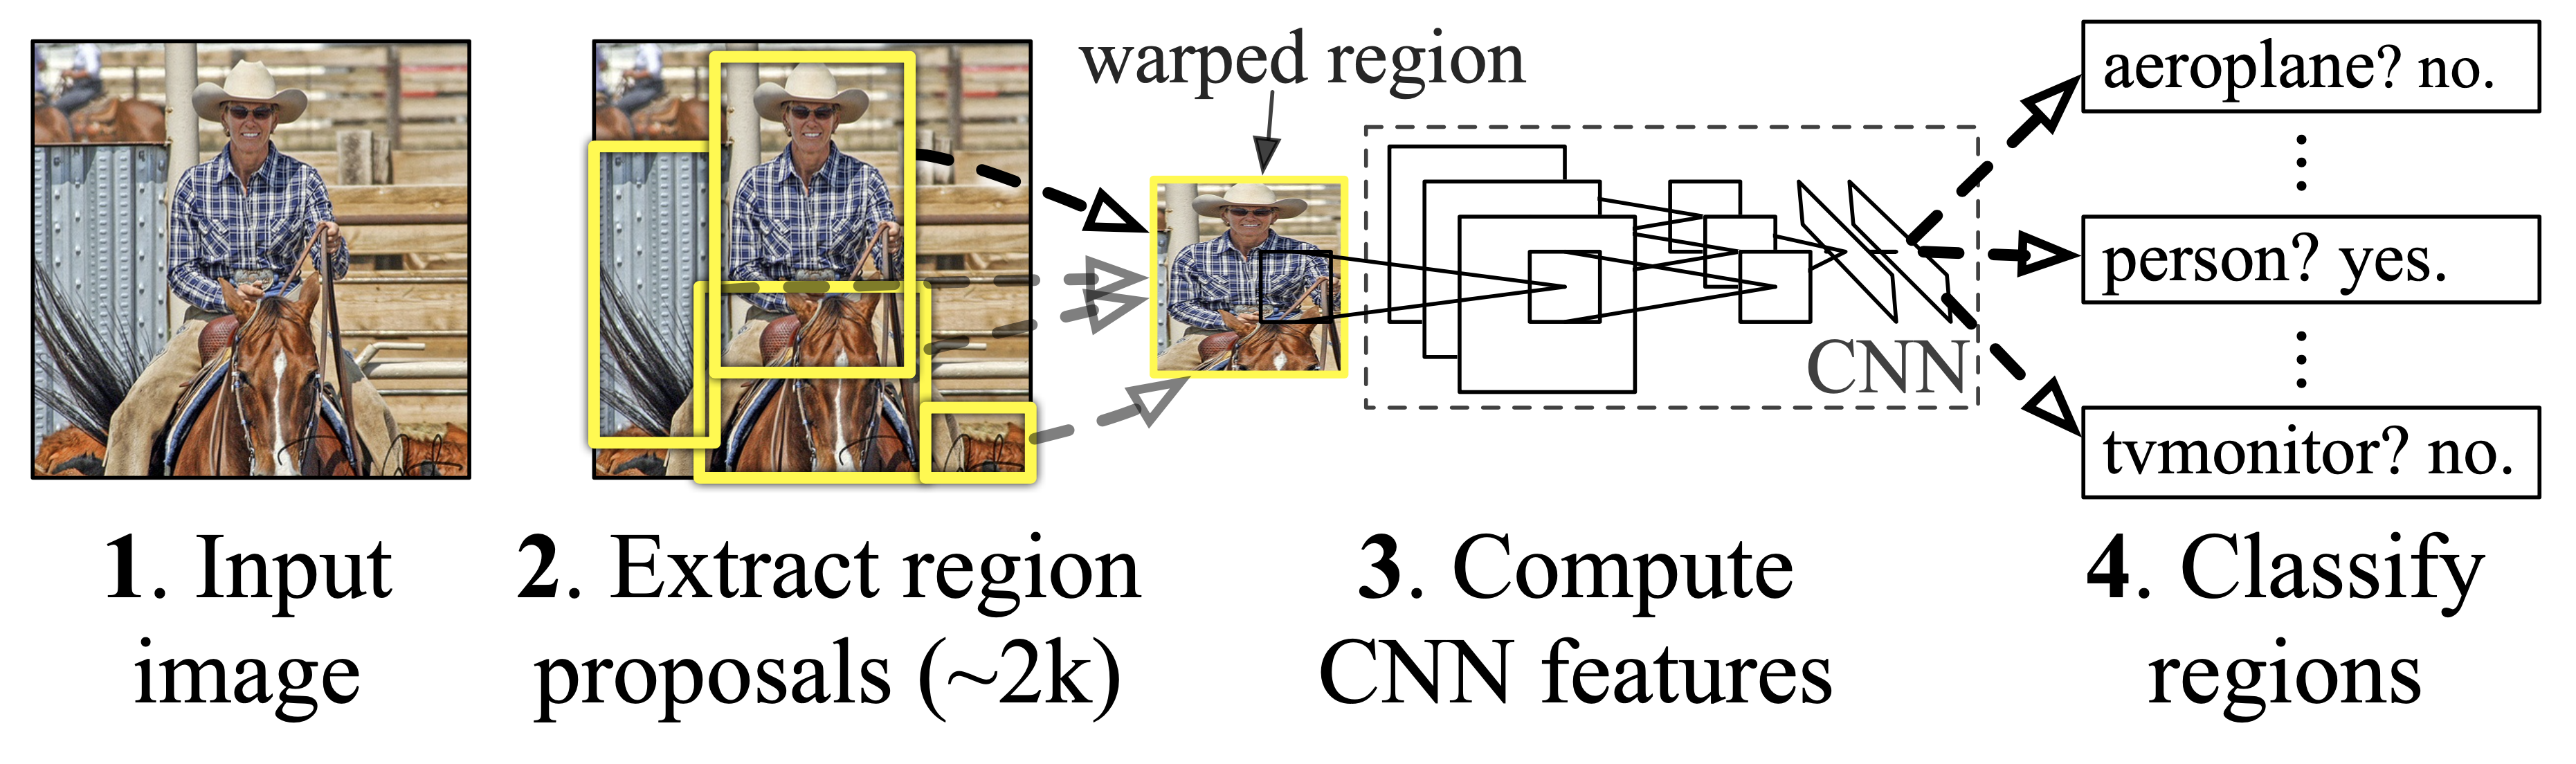
\includegraphics[height=2cm,keepaspectratio]{images/2_literature/r-cnn.png}
\end{center}
\caption{R-CNN: Object detection overview \cite{Girshick2013}.}
\end{figure}

\subsubsection{Fast R-CNN}
The initial R-CNN model worked, but it was quite slow. This slowdown was because each of the 2000 extracted regions, was passed through the CNN. The same author continued his research to solve this problem. His new model was called Fast R-CNN \cite{Girshick2015}. Instead of passing each region through a CNN, the full image is passed through. The generated regions are then projected on the feature map generated by the CNN. The resulting projection is known as ``Region of Interest'' (ROI). Additionally, with Fast R-CNN, the SVM classifier is replaced with fully connected layers. The original R-CNN takes about 50 seconds per image to detect objects, whereas the Fast version was able to process the image in 2 seconds.

\begin{figure}[ht]
\begin{center}
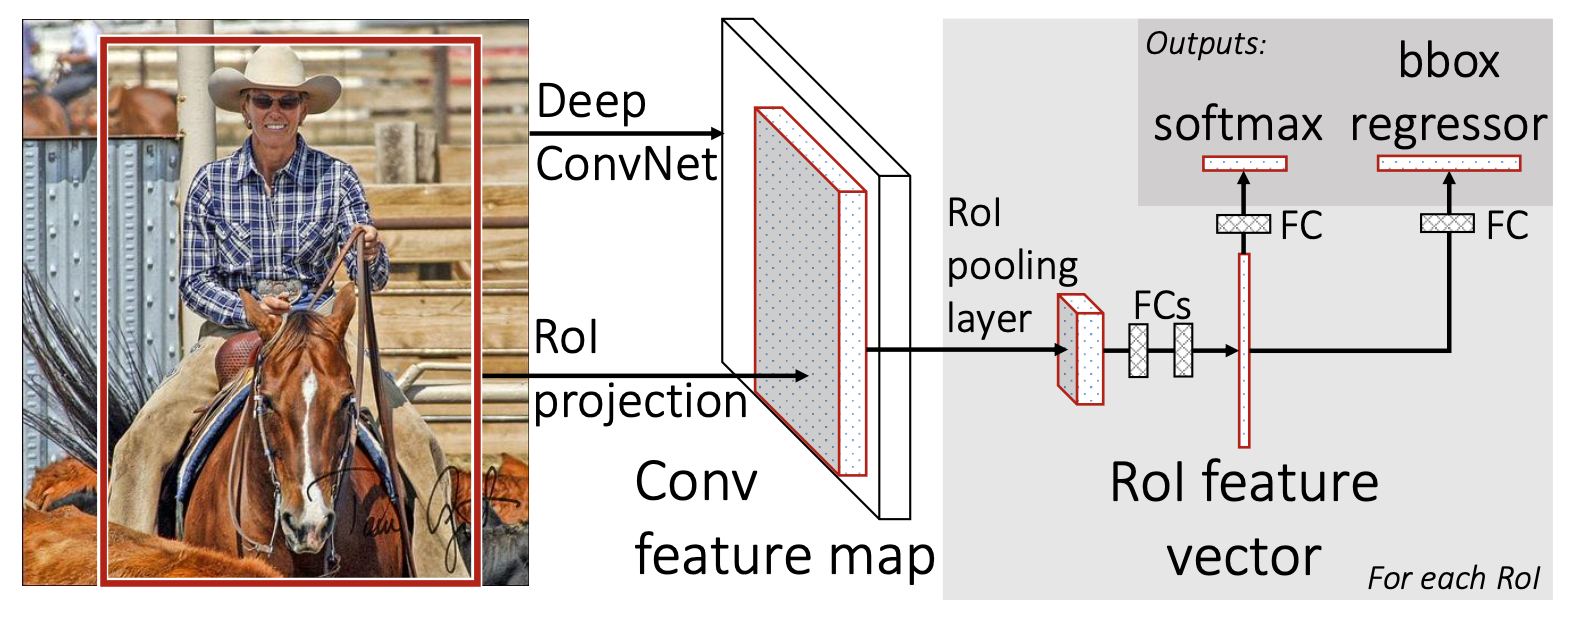
\includegraphics[height=2cm,keepaspectratio]{images/2_literature/fast-r-cnn.png}
\end{center}
\caption{Fast R-CNN: Object detection overview \cite{Girshick2015}.}
\end{figure}

\subsubsection{Faster R-CNN}
Although Fast R-CNN is significantly quicker to detect objects, it still takes about 2 seconds to localize the object. The bottleneck now was the region proposal algorithm, which is implemented on the CPU. Improvements over the used selective search were researched. However, \authorref{Ren2015} argued that it would be more interesting to develop a model which combines region proposal and object detection. Their model was called Faster R-CNN and is able to process an image in 200 milliseconds. 

Faster R-CNN consists of two modules. The first module is a deep fully convolutional network which proposes regions, known as Region Proposal Network (RPN). The RPN takes an image as input and outputs a set of object proposals, each with an \textit{objectness score} (measurement if something is an object or background). This output is fed into the second module, which is the Fast R-CNN object detector. 

The unified model has several advantages over the Fast R-CNN model. Because the region proposal are generated within the network, the model can be trained end-to-end. Making deployment easier, requires less resources, and performs much faster. Additionally, this allows the region proposals to be tuned according to the detection task.


\begin{figure}[ht]
\begin{center}
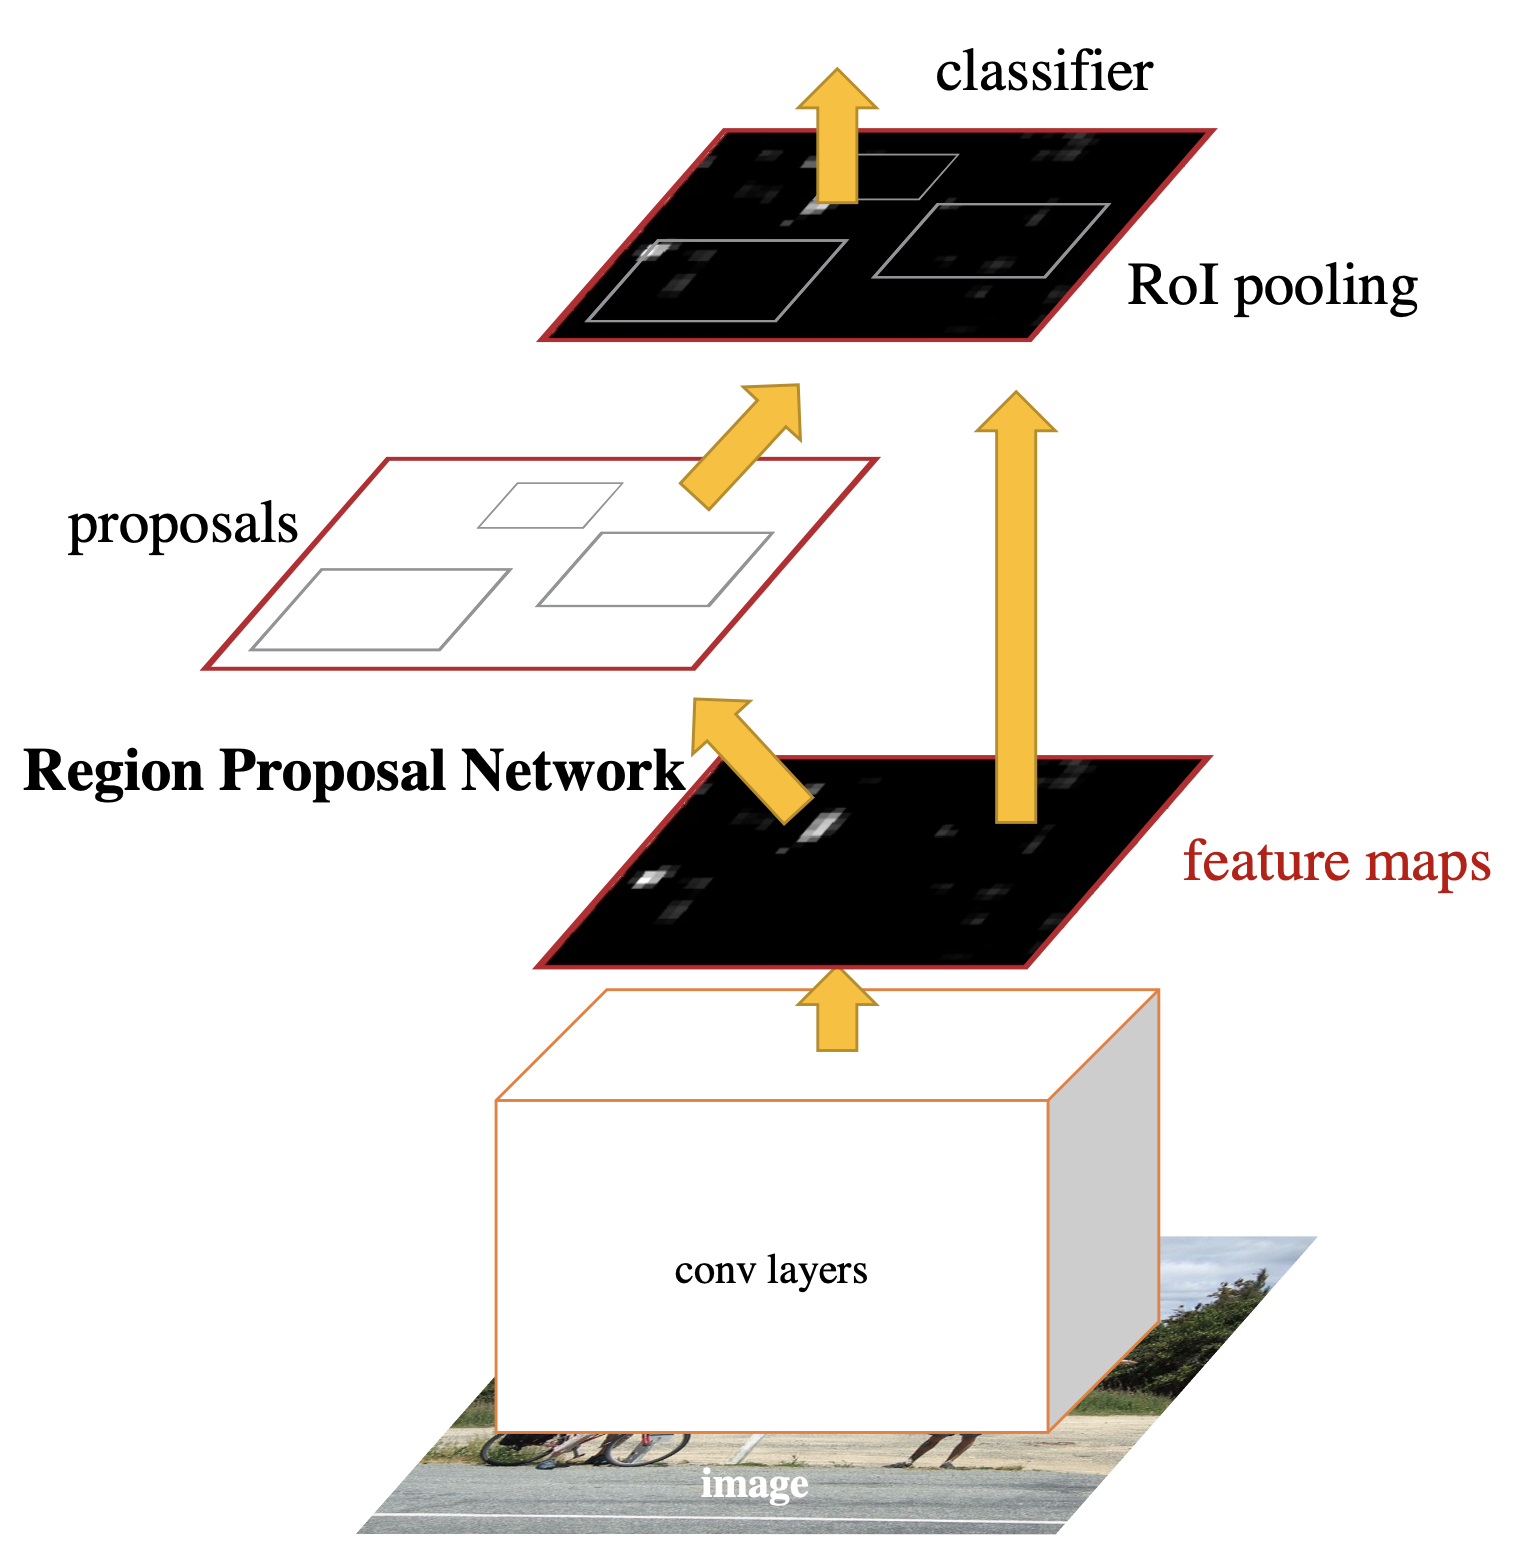
\includegraphics[height=5cm,keepaspectratio]{images/2_literature/faster-r-cnn.png}
\end{center}
\caption{Faster R-CNN: Object detection overview \cite{Ren2015}.}
\end{figure}


\subsubsection{YOLO}
The previous detectors all use regions to localize an object. The models look at parts of the image with high probability of containing an object. YOLO has a different architecture by looking at the complete image. A single neural network predicts bounding boxes and class probabilities in one evaluation. Using the system, ``you only look once'' (YOLO) at an image to see what objects it contains \authorref{Redmon2016}.

YOLO as several benefits. First of all is that YOLO is extremely fast. Due the new architecture, it doesn't require a complex pipeline, and can be trained end-to-end. Secondly, unlike previous models, YOLO reasons globally about the image. Most mistakes from earlier models are due mistaking background for an object. YOLO makes less than half the number of background errors compared to Fast R-CNN. Finally, YOLO is capable to learn generalizable representations of objects. For instance, when YOLO is trained on natural images and tested on art-work, YOLO outperforms top detectors such as R-CNN. YOLO does lag behind state-of-the-art detectors in terms of accuracy. Although it can quickly detect objects, its struggles to precisely localize small objects.

YOLO works by taking an image and split it into an SxS grid. Each grid predicts B bounding boxes, and a confidence scores for those boxes. These scores reflect how confident the model is that the box contains an object. The model outputs for each bounding box 5 predictions: the location (x, y), size (w, h) and confidence score. Additionally, each grid cell also predicts C conditional class probabilities. The complete output is then passed through a deep convolution neural network to make detections. 

\begin{figure}[ht]
\begin{center}
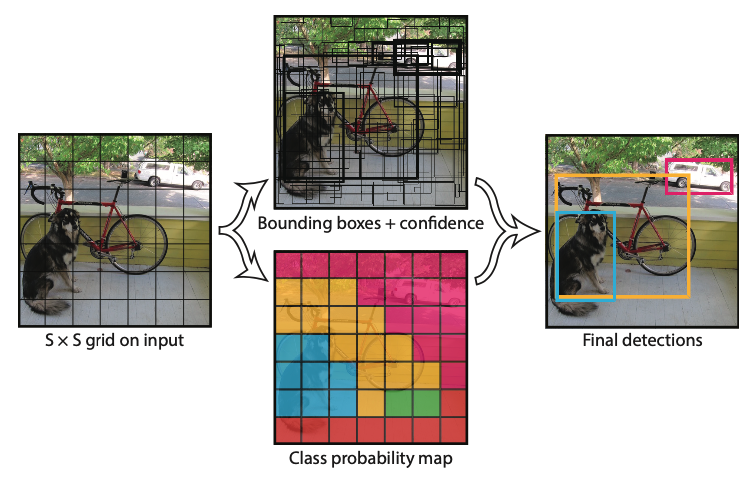
\includegraphics[width=10cm,keepaspectratio]{images/2_literature/yolo.png}
\end{center}
\caption{You Ony Look Once (YOLO) detector model \cite{Redmon2016}.}
\end{figure}


\subsubsection{YOLOv2}
The authors of YOLO continued their work and introduce two new detectors YOLOv2 and YOLO9000 \cite{Redmon2017}. They argue that current object detection datasets are limited (contain about hundred thousand images) compared to datasets used for classification and tagging (contain about millions of images with thousands of categories). They propose a novel method to harness large amount classification data and use it to expand current detection systems. Using this method they develop YOLO9000, a real-time object detector that can detect over 9000 categories. To do so, they first improve the base YOLO detection system to produce YOLOv2. 

YOLO suffers from various shortcomings relative to state-of-the-art detection systems. YOLO makes significantly number of localization errors compared to Fast R-CNN. In deep-learning, better performance often comes from training larger networks or ensambling networks together. With YOLO, the authors opt to simplify the network and introduce several architectural changes. In short, most improvements stem by implementing state-of-the-art deep learning techniques. As the details are not relevant for this work, please refer for details to \cite{Redmon2017}.  Below is shown an comparison of accuracy and speed between various detectors to demonstrate the effects.


\subsubsection{YOLOv3}
YOLOv3 is another improved version of YOLO by the same authors \cite{Redmon2018}. It uses a new base model which is a bit slower but more accurate. YOLOv3 predicts boxes at 3 different scales, based on the idea of Feature Pyramid Network \cite{Lin2017}. This allows the model to learn objects at different scales. Remedying the problem with detection of small objects. Additionally, YOLOv3 performs multi-label classification instead of earlier used softmax. This makes it possible to label the same object with multiple labels, e.g., an object can be both a person and a woman.


\begin{figure}[ht]
\begin{center}
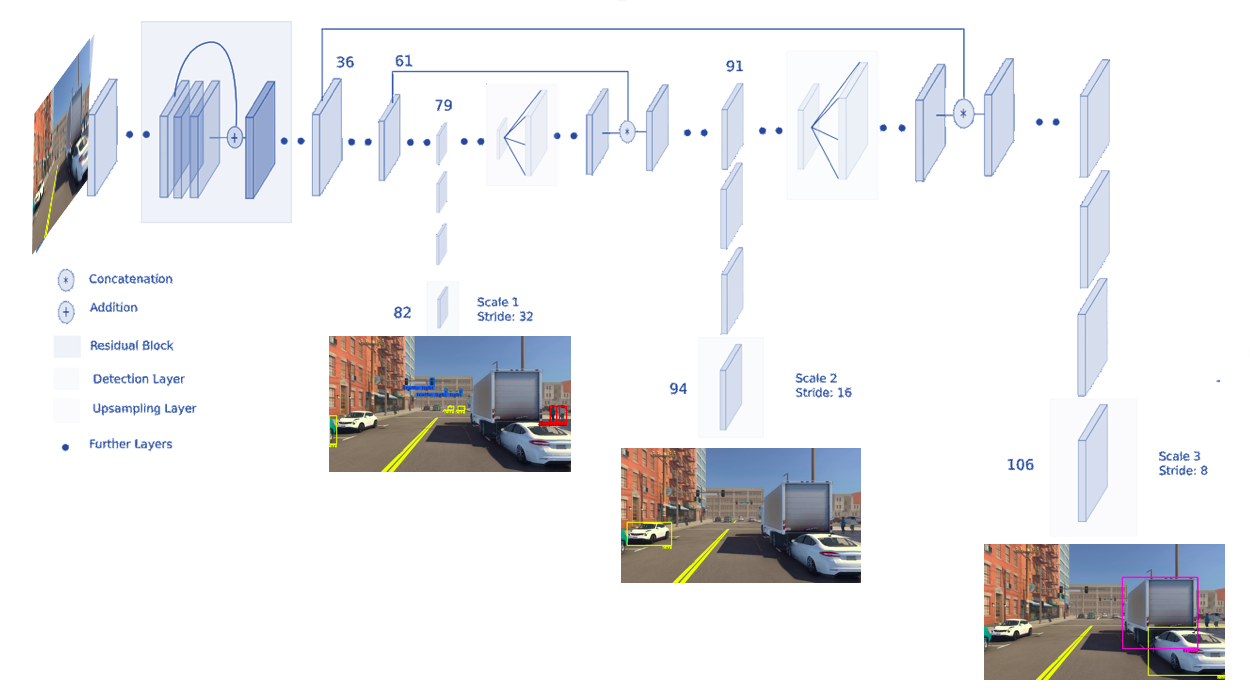
\includegraphics[width=14cm,keepaspectratio]{images/2_literature/yolov3-architecture.png}
\end{center}
\caption{YOLOv3 network architecture \cite{Dulepet2020}. Note that based on the output scale, the model detects objects of different sizes.}
\end{figure}


\subsubsection{YOLOv4}

YOLOv4 is the successor of YOLOv3. Unlike earlier models, YOLOv4 is developed by other authors \authorref{Bochkovskiy2020}. In their paper the authors explore various deep learning techniques to improve the performance of YOLO, some deriving from earlier research, as well some novel techniques. The results is an improvement of 10\% accuracy and about 12\% increase in speed.

One of these novel techniques is named Mosaic. It is a data augmentation method that mixes 4 training images. Thus mixing 4 different contexts. This allows detection of objects outside their normal context. In addition, when applying batch normalization, it calculates statistics from 4 different images. Reducing the need for large mini-batch sizes.

Another novel technique is Self-Adversarial Training (SAT). This is also a data augmentation technique that operates in 2 stages. In the first stage, the network modifies the image instead of the weights. Thereby performing an adversarial attack on itself. In the second stage, the network is trained to detect an object on this modified image.


\subsubsection{YOLOv5}
Currently, there is no paper released on YOLOv5. At this time, it seems that YOLOv5 is still under active development \cite{Jocher2021}. Nevertheless, the authors claim it outperforms all current object detectors. In the Road Damage Competition \cite{Arya2020-competition}, YOLOv5 it was already used in the winning model \cite{rddc2020}. In this work YOLOv5 is also used. In figure \ref{fig:yolo-architecture} we can see the neural network architecture. 

The authors provide various pretrained configurations of the model. The overall architecture remains the same but each configuration differs in the network size. For instance, the small \code{YOLOv5s} has 7.2 million parameters and the larger \code{YOLOv5m} has 21.2 million parameters. Each model is pretrained on the COCO dataset \cite{COCO}. This is a benchmark dataset used for object detection. It contains thousands of images for 80 different classes.

\begin{figure}[ht]
\begin{center}
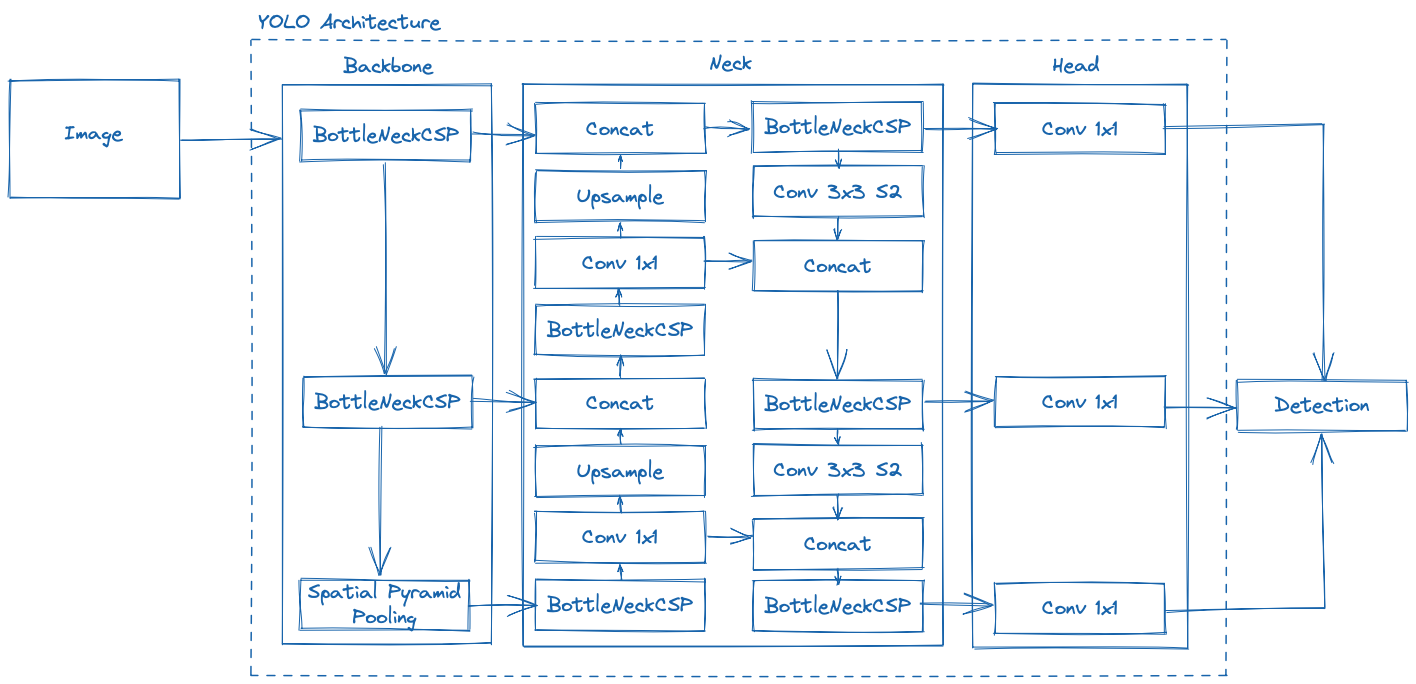
\includegraphics[width=0.95\textwidth,keepaspectratio]{images/2_literature/yolo-architecture.png}
\end{center}
\captionsetup{width=.90\textwidth}
\caption{Architecture of the YOLOv5 network. It is derived from the source code \cite{Jocher2021}.}
\label{fig:yolo-architecture}
\end{figure}


% \subsection{Accelerometer Signal Processing}
% From literature on detecting road defects using accelerometer data, we find that there are certain processing operations typically performed. In this section, we explain these common operations as they will be used in our pipeline as well.


\subsection{Fast Fourier Transform}
\label{sec:fft}

Fourier analysis converts a signal from its original domain (often time or space) to a representation in the frequency domain. Fast Fourier Transform (FFT) is an algorithm that computes the periodic components by convoluting sine waves having different frequencies with the signal \cite{Cooley1965}. Basically, it describes the original signal as combination of many periodic sine waves. The output of the algorithm is known as the frequency spectrum. It tells us all the frequencies that are present and in what proportion. The inverse Fourier Transform constructs a signal given the periodic signals. 

The Fourier Transform has many uses in signal processing. For instance, convolution in the time domain is equal to multiplication in the frequency domain. For discrete signals it is almost always faster to implement the convolution from the frequency domain. Finally, in the research of detecting potholes using accelerometer, the frequency spectrum is used as feature extraction \cite{Wu2020}.


% \subsection{Cross Correlation}
% \label{sec:cross-correlation}

% As mentioned earlier in section \ref{section:multimodal-ml}, cross-correlation is often used to synchronize two signals \cite{Knapp1976}. The original approach is rather expensive to compute, with a complexity of $O(n^2)$. Fortunately, cross correlation can also be computed using a more efficient approach based on FFT. The latter approach has a complexity of only $O(n \log n)$ \cite{Lewis2001}. Cross correlation is defined as follows.

% \begin{align*}
% R(\tau) = \int x(t) y(t + \tau) dt 
% \end{align*}

% Where $x(t)$ and $y(t)$ are the input signals, both a function of time. $\tau$ is the time delay, and R is the cross correlation, a function of time delay $\tau$. The optimal time shift for synchronizing both streams is computed by choosing the $\tau$ that maximizes the cross correlation. 

% In this thesis synchronization of the sensors presents some challenges. Often it is sufficient to synchronize the capture time of the sensors. However in our case, the camera looks ahead, and we want to find the delay total $\tau = \tau_{capture} + \tau_{detection}$ between a detected object and when the vehicle travels over that object. Refer back to figure \ref{fig:synchronization} for illustration. With cross-correlation we calculate the delay $\tau_{capture}$. To calculate $\tau_{detection}$, a novel approach is developed in \ref{sec:object-distance}.

% Calculating the $\tau_{detection}$ is more challenging. The delay depends on when the object is detected in the image, i.e., might be closer or further, and the travelling speed. In theory, we could overcome this issue if know the distance of the object to the vehicle and traveling speed. Calculating the distance of object to the vehicle is possible if we calibrate the visual signal. This calibration needs to be performed every time the smartphone is re-positioned. As it is unlikely that the smartphone is replaced consistently with the same angle at all times, a novel approach is developed in section \ref{sec:object-distance}.


\subsection{Butterworth Filter}
\label{sec:butterworth-filter}

Accelerometer data is prone to noise. As is common with signal processing, data is first passed through a filter to obtain a clearer signal. Digital filter operates on sampled, discrete-time signal (i.e., time series) to reduce or enhance certain aspects of that signal. One of the most commonly used filters is the Butterworth filter. It is filter which operates in the frequency domain. It is designed to have frequency response that is as flat as possible in the ``passband''. The pass-band is the range of frequencies that are allowed to pass i.e., not filtered. For instance, a low-pass filter only allow allows frequencies in the signal below a certain threshold. This threshold in signal processing is known as the cutoff frequency.

Existing research on detecting potholes uses a variety of different filter configurations to clean the data. Some apply a low-pass Butterworth filter \cite{Gupta2020}, whereas other researches use a high-pass Butterworth filter \cite{Wu2020, Janani2020}. Due the different usages, we assume that it differs per application and approach it as a possible tuning parameter.


% Another key challenge for our data collection is partial observability. Partial observability refers to the fact that the same phenomena may not always be captured by both sensors. This happens because the field-of-view of the camera is much wider than that of the accelerometer. While the accelerometer can only detect a defect when the wheel of the vehicle travels over said defect. This is also visualized in figure \ref{fig:sensor-delay}.

% \begin{figure}[ht]
% \begin{center}
% 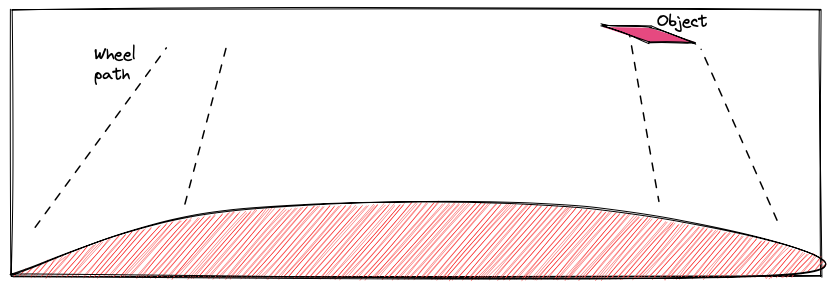
\includegraphics[width=0.95\textwidth,keepaspectratio]{images/2_literature/partial-observability.png}
% \end{center}
% \captionsetup{width=.90\textwidth}
% \caption{Illustration of the partial observability problem: objects in the accelerometer data can only be detected when the wheels of the vehicle drives over that object.}
% \end{figure}



% \textbf{External trigger}
% One method to overcome this issue is using an external trigger to align the modalities. For instance in \cite{Cippitelli2015}, the authors are able to time synchronize visual data by calculating the delay when a controlled trigger is visible. 

% https://www.coursera.org/lecture/state-estimation-localization-self-driving-cars/lesson-2-multisensor-fusion-for-state-estimation-2imn3
